%
%      This is an example of an elaborate TikZ plot
%      to show possibilities 
%

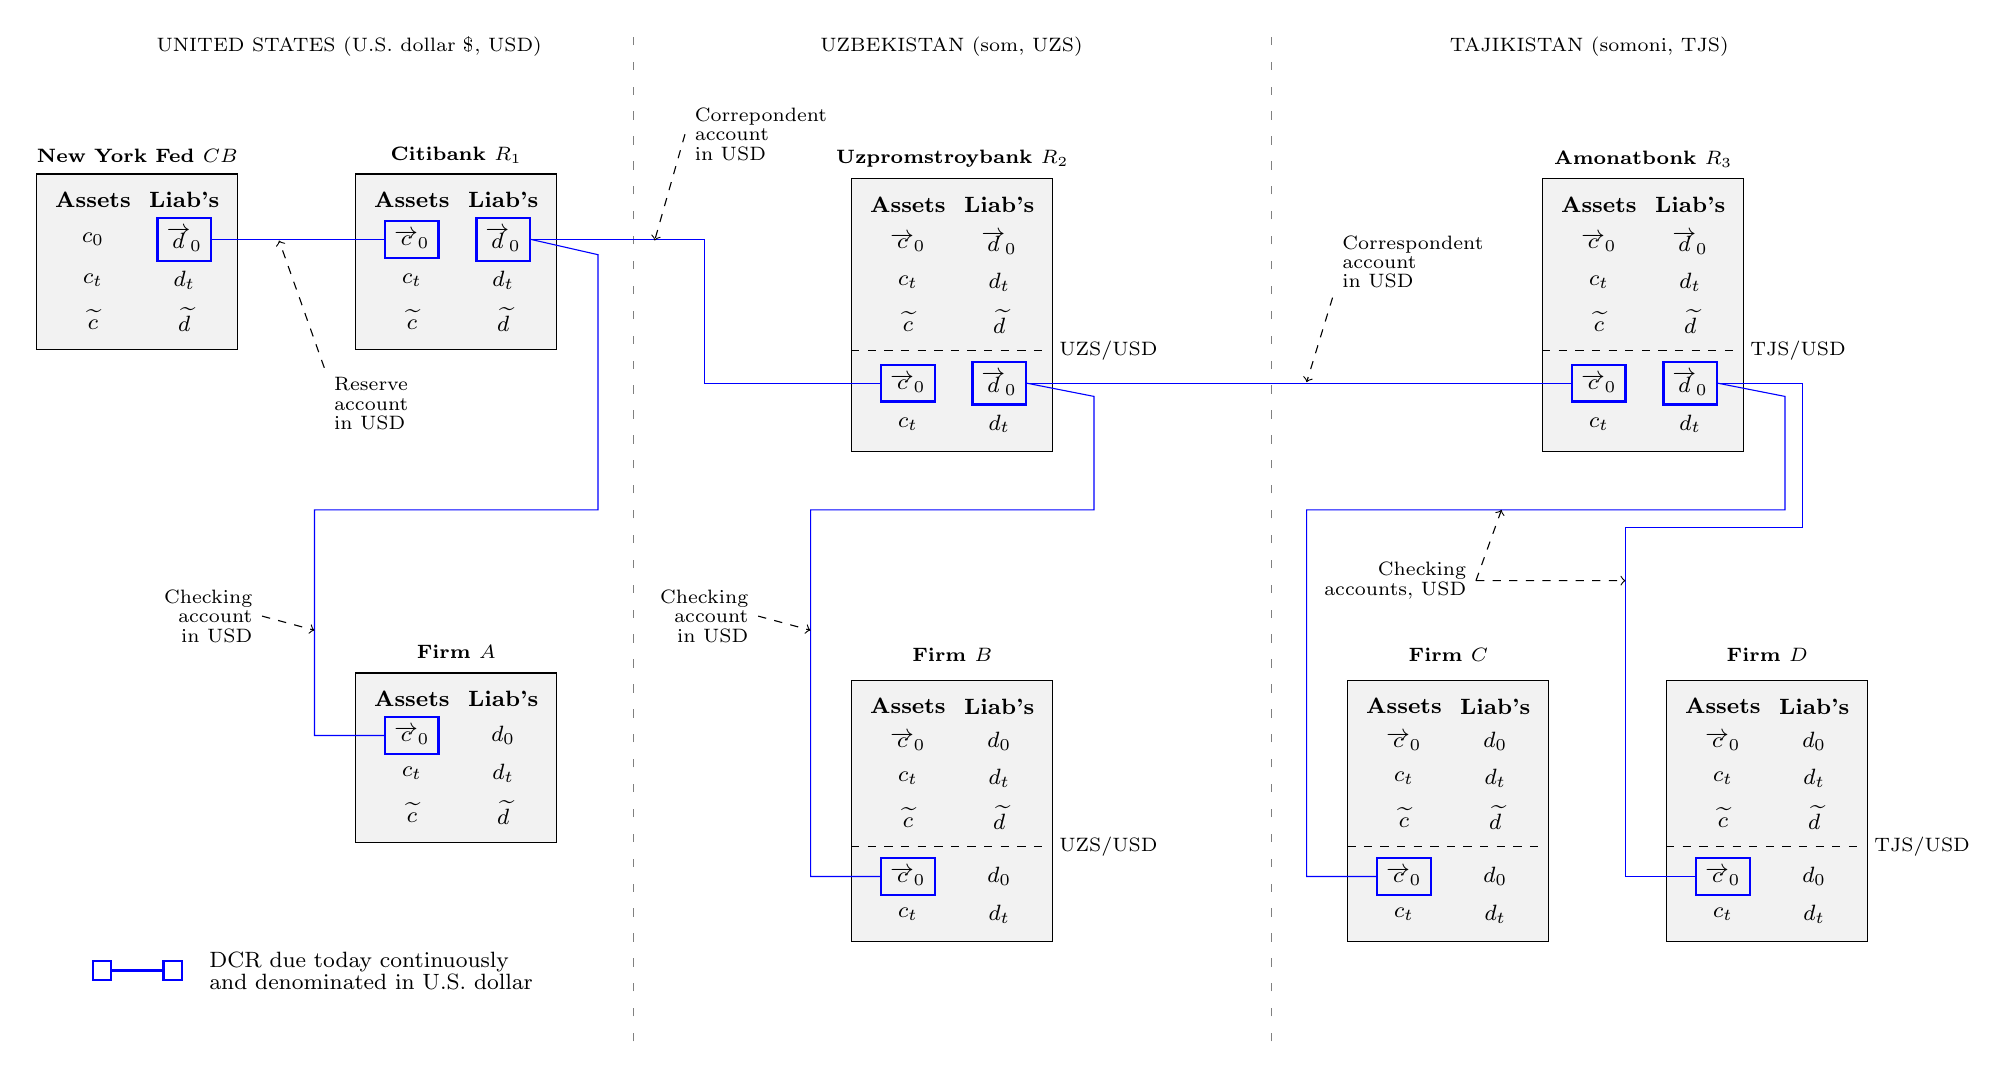
\begin{tikzpicture}[scale=.9]
    \draw[help lines,white] (0,0) grid (26,14);
    \draw[gray,loosely dashed] (8.5,0) -- (8.5,14.25); 
    \draw[gray,loosely dashed] (17.5,0) -- (17.5,14.25); 
    \node[black]  at (4.5,14) {\textsuperscript{\MakeUppercase{United States} (U.S. dollar \$, USD)}};
    \node[black] at (13,14) {\textsuperscript{\MakeUppercase{Uzbekistan} (som, UZS)}};
    \node[black] at (22,14) {\textsuperscript{\MakeUppercase{Tajikistan} (somoni, TJS)}};
    \draw[blue,thick] (1,1) node(a)[draw] {} (2,1) node(b)[draw] {};
    \draw[blue,thick] (a) -- (b);
    \node[black,align=left,font=\fontsize{8}{8}\selectfont] at (4.8,1)%
        {DCR due today continuously\\and denominated in U.S. dollar};
    % United States ====================================================
    % NY Fed ----------------------------------------------------------
        \node [matrix,fill=gray!10,draw=black,thin,font=\bf\fontsize{8}{8}\selectfont] (CB) at (1.5,11) {
            \node {Assets}; & \node {Liab's}; \\
            \node {$c_0$}; & \node[rectangle,draw=blue,thick] (CB_d0)  {$\overrightarrow{d}_0$}; \\
            \node {$c_t$}; & \node {$d_t$}; \\
            \node {$\widetilde{c}$}; & \node {$\widetilde{d}$}; \\
            };
        \draw (CB)++(0,1.5) node[font=\bf\fontsize{7}{7}\selectfont]%
            {New York Fed $CB$};
    % Citibank ----------------------------------------------------------
        \node [matrix,fill=gray!10,draw=black,thin,font=\bf\fontsize{8}{8}\selectfont] (R1) at (6,11) {
            \node {Assets}; & \node {Liab's}; \\
            \node[rectangle,draw=blue,thick] (R1_c0) {$\overrightarrow{c}_0$}; & \node[rectangle,draw=blue,thick] (R1_d0)  {$\overrightarrow{d}_0$}; \\
            \node {$c_t$}; & \node {$d_t$}; \\
            \node {$\widetilde{c}$}; & \node {$\widetilde{d}$}; \\
            };
        \draw (R1)++(0,1.5) node[font=\bf\fontsize{7}{7}\selectfont]%
            {Citibank $R_1$};
    % Firm A ----------------------------------------------
    \node [matrix,fill=gray!10,draw=black,thin,font=\bf\fontsize{8}{8}\selectfont] (A) at (6,4) {
            \node {Assets}; & \node {Liab's}; \\
            \node[rectangle,draw=blue,thick] (A_c0) {$\overrightarrow{c}_0$}; & \node {$d_0$}; \\
            \node {$c_t$}; & \node {$d_t$}; \\
            \node {$\widetilde{c}$}; & \node {$\widetilde{d}$}; \\
            };
        \draw (A)++(0,1.5) node[font=\bf\fontsize{7}{7}\selectfont]%
            {Firm $A$};
    \draw[blue] (CB_d0) -- (R1_c0);
    \draw[blue] (A_c0.west) -| (4,6) -- (4,7.5) -- (8,7.5) -- (8,11.1) -- (R1_d0.east);
    % Uzbekistan ====================================================
    % Uzromstroybank ------------------------------------------------------------
        \node [matrix,fill=gray!10,draw=black,thin,font=\bf\fontsize{8}{8}\selectfont] (R2) at (13,10.25) {
            \node {Assets}; & \node {Liab's}; \\
            \node {$\overrightarrow{c}_0$}; & \node {$\overrightarrow{d}_0$}; \\
            \node {$c_t$}; & \node {$d_t$}; \\
            \node {$\widetilde{c}$}; & \node {$\widetilde{d}$}; \\
            \node {}; & \node {}; \\
            \node[rectangle,draw=blue,thick] (R2_c0) {$\overrightarrow{c}_0$}; & \node[rectangle,draw=blue,thick] (R2_d0) {$\overrightarrow{d}_0$}; \\
            \node {$c_t$}; & \node {$d_t$}; \\
            };
        \draw[dashed] (R2.west)++(0,-.5) -- +(2.8,0) node[at end,right,font=\fontsize{7}{7}\selectfont] {UZS/USD};
        \draw (R2)++(0,2.2) node[font=\bf\fontsize{7}{7}\selectfont]%
            {Uzpromstroybank $R_2$};
    % Firm B ----------------------------------------------
    \node [matrix,fill=gray!10,draw=black,thin,font=\bf\fontsize{8}{8}\selectfont] (B) at (13,3.25) {
            \node {Assets}; & \node {Liab's}; \\
            \node {$\overrightarrow{c}_0$}; & \node {$d_0$}; \\
            \node {$c_t$}; & \node {$d_t$}; \\
            \node {$\widetilde{c}$}; & \node {$\widetilde{d}$}; \\
            \node {}; & \node {}; \\
            \node[rectangle,draw=blue,thick] (B_c0) {$\overrightarrow{c}_0$}; & \node {$d_0$}; \\
            \node {$c_t$}; & \node {$d_t$}; \\
            };
        \draw[dashed] (B.west)++(0,-.5) -- +(2.8,0) node[at end,right,font=\fontsize{7}{7}\selectfont] {UZS/USD};
        \draw (B)++(0,2.2) node[font=\bf\fontsize{7}{7}\selectfont]%
            {Firm $B$};
    \draw[blue] (R1_d0) -| (9.5,11) |- (R2_c0);
    \draw[blue] (B_c0.west) -| (11,4) -- (11,7.5) -- (15,7.5) -- (15,9.1) -- (R2_d0.east);
    % Tajikistan ====================================================
    % Amonatbonk ----------------------------------------------------------
        \node [matrix,fill=gray!10,draw=black,thin,font=\bf\fontsize{8}{8}\selectfont] (R3) at (22.75,10.25) {
            \node {Assets}; & \node {Liab's}; \\
            \node {$\overrightarrow{c}_0$}; & \node {$\overrightarrow{d}_0$}; \\
            \node {$c_t$}; & \node {$d_t$}; \\
            \node {$\widetilde{c}$}; & \node {$\widetilde{d}$}; \\
            \node {}; & \node {}; \\
            \node[rectangle,draw=blue,thick] (R3_c0) {$\overrightarrow{c}_0$}; & \node[rectangle,draw=blue,thick] (R3_d0) {$\overrightarrow{d}_0$}; \\
            \node {$c_t$}; & \node {$d_t$}; \\
            };
        \draw[dashed] (R3.west)++(0,-.5) -- +(2.8,0) node[at end,right,font=\fontsize{7}{7}\selectfont] {TJS/USD};
        \draw (R3)++(0,2.2) node[font=\bf\fontsize{7}{7}\selectfont]%
            {Amonatbonk $R_3$};
    \draw[blue] (R2_d0) -- (R3_c0);
    % Firm C ----------------------------------------------
    \node [matrix,fill=gray!10,draw=black,thin,font=\bf\fontsize{8}{8}\selectfont] (C) at (20,3.25) {
            \node {Assets}; & \node {Liab's}; \\
            \node {$\overrightarrow{c}_0$}; & \node {$d_0$}; \\
            \node {$c_t$}; & \node {$d_t$}; \\
            \node {$\widetilde{c}$}; & \node {$\widetilde{d}$}; \\
            \node {}; & \node {}; \\
            \node[rectangle,draw=blue,thick] (C_c0) {$\overrightarrow{c}_0$}; & \node {$d_0$}; \\
            \node {$c_t$}; & \node {$d_t$}; \\
            };
        \draw[dashed] (C.west)++(0,-.5) -- +(2.8,0) node[at end,right,font=\fontsize{7}{7}\selectfont] {};
        \draw (C)++(0,2.2) node[font=\bf\fontsize{7}{7}\selectfont]%
            {Firm $C$};
    % Firm D ----------------------------------------------
    \node [matrix,fill=gray!10,draw=black,thin,font=\bf\fontsize{8}{8}\selectfont] (D) at (24.5,3.25) {
            \node {Assets}; & \node {Liab's}; \\
            \node {$\overrightarrow{c}_0$}; & \node {$d_0$}; \\
            \node {$c_t$}; & \node {$d_t$}; \\
            \node {$\widetilde{c}$}; & \node {$\widetilde{d}$}; \\
            \node {}; & \node {}; \\
            \node[rectangle,draw=blue,thick] (D_c0) {$\overrightarrow{c}_0$}; & \node {$d_0$}; \\
            \node {$c_t$}; & \node {$d_t$}; \\
            };
        \draw[dashed] (D.west)++(0,-.5) -- +(2.8,0) node[at end,right,font=\fontsize{7}{7}\selectfont] {TJS/USD};
        \draw (D)++(0,2.2) node[font=\bf\fontsize{7}{7}\selectfont]%
            {Firm $D$};
    \draw[blue] (C_c0.west) -| (18,4) -- (18,7.5) -- (24.75,7.5) -- (24.75,9.1) -- (R3_d0.east);
    \draw[blue] (D_c0.west) -| (22.5,4) -- (22.5,7.25) -- (25,7.25) -- (25,9.1) |- (R3_d0.east);
    % Labels
    \node[align=right,font=\fontsize{7}{7}\selectfont] (t) at (2.5,6) {Checking\\account\\in USD};
    \draw[->,dashed] (t.east) -- (4,5.8);
    \node[align=right,font=\fontsize{7}{7}\selectfont] (t) at (9.5,6) {Checking\\account\\in USD};
    \draw[->,dashed] (t.east) -- (11,5.8);
    \node[align=right,font=\fontsize{7}{7}\selectfont] (t) at (19.25,6.5) {Checking\\accounts, USD};
    \draw[->,dashed] (t.east) -- (20.75,7.5); \draw[->,dashed] (t.east) -- (22.5,6.5);
    \node[align=left,font=\fontsize{7}{7}\selectfont] (t) at (4.8,9) {Reserve\\account\\in USD};
    \draw[->,dashed] (t.north west) -- (3.5,11.3);
    \node[align=left,font=\fontsize{7}{7}\selectfont] (t) at (10.3,12.8) {Correpondent\\account\\in USD};
    \draw[->,dashed] (t.west) -- (8.8,11.3);
    \node[align=left,font=\fontsize{7}{7}\selectfont] (t) at (19.5,11) {Correspondent\\account\\in USD};
    \draw[->,dashed] (t.south west) -- (18,9.3);
\end{tikzpicture}
